\documentclass[a4paper, titlepage, twoside, openright, french]{report}

\usepackage[utf8]{inputenc}
\usepackage[T1]{fontenc}
\usepackage{babel}

\usepackage{xcolor}
\usepackage{adjustbox}

\usepackage{xspace}

\usepackage{listings}
\usepackage{lstautogobble}

\usepackage{booktabs}
\usepackage{makecell}

\usepackage{fullpage}

\usepackage[hidelinks]{hyperref}

\usepackage{makeidx}
\makeindex
\usepackage[intoc]{nomencl}
\makenomenclature

\usepackage{amsmath}
\usepackage{amsthm}
\usepackage{amssymb}
\usepackage{mathtools}

\newcommand{\N}{\mathbb{N}\xspace}

\renewcommand{\epsilon}{\varepsilon}
\renewcommand{\phi}{\varphi}

\allowdisplaybreaks % Autorise les environnements à faire un page break

% J'ai suivi les recommandations de http://mirror.koddos.net/CTAN/macros/latex/required/amscls/doc/amsthdoc.pdf
\theoremstyle{plain}
\newtheorem{thm}{Théorème}[section]
\newtheorem{theorem}[thm]{Théorème} % Parce qu'à chaque fois, je me trompe
\newtheorem{lemme}{Lemme}[section]
\newtheorem{corollaire}{Corollaire}[section]

\theoremstyle{definition}
\newtheorem{definition}{Définition}[section]
\newtheorem{propriete}{Propriété}[section]
\newtheorem{exemple}{Exemple}[section]

\theoremstyle{remark}
\newtheorem{note}{Note}[section]
\newtheorem{rem}{Remarque}[section]
\newtheorem{remarque}[rem]{Remarque}
\newtheorem{illustration}{Illustration}[section]

\newenvironment{demonstration}{\begin{proof}[\textnormal{\textbf{Preuve}}]}{\end{proof}}
\newenvironment{preuve}{\begin{demonstration}}{\end{demonstration}\ignorespacesafterend}

% Traductions
\newcommand{\thmautorefname}{Théorème}
\renewcommand{\theoremautorefname}{Théorème}
\newcommand{\proprieteautorefname}{Propriété}
\newcommand{\exempleautorefname}{Exemple}
\newcommand{\lemmeautorefname}{Lemme}
\newcommand{\definitionautorefname}{Définition}
\newcommand{\algorithmautorefname}{Algorithme}
\usepackage[explicit]{titlesec}
\usepackage{chngcntr}

\counterwithin{figure}{section} % Pour que les figures soient numérotées en fonction du chapitre.section.numéro
\counterwithin{equation}{section}

% Numérotation des sous-sous-sections
\setcounter{secnumdepth}{3}
\usepackage{tikz}
\usetikzlibrary{arrows, shapes, calc, positioning, external}

\tikzexternalize
\tikzsetexternalprefix{figures/}

\tikzset {
    sum/.style = {
        draw,
        shape = circle,
        font={$\Sigma$} % Small hack to set \Sigma in every sum node
    },
    Z/.style = {
        draw,
        shape = rectangle,
        minimum width=25pt,
        minimum height=20pt,
        font = {$z^{-1}$} % To set z^{-1} in every Z node
    },
    multiply/.style args = {#1}{
        draw,
        regular polygon,
        regular polygon sides = 3,
        inner sep=0pt,
        minimum size=25pt,
        label = {[label distance=0.1cm]#1}
    },
    multiply right/.style args = {#1}{
        multiply={#1},
        shape border rotate=-90,
    },
    multiply left/.style args = {#1}{
        multiply={#1},
        shape border rotate=90,
    },
    branch/.style = {
        draw,
        shape = circle,
        fill,
        inner sep=0pt,
        minimum size=4pt
    },
    every path/.style = {
        ->,
        >=stealth',
        line width=1pt,
        draw
    }
}
\usepackage{fancyhdr}
\pagestyle{fancy}
\usepackage{emptypage}

\setlength{\headheight}{15pt}
\setlength{\headsep}{0.2cm}

\renewcommand{\chaptermark}[1]{\markboth{\thechapter. #1}{}}
\renewcommand{\sectionmark}[1]{\markright{\thesection. #1}{}}

\fancyhf{} % supprime les en-têtes et pieds prédéfinis
\fancyhead[R]{\thepage} % Met le numéro de la page à droite sur toutes les pages
\fancyhead[LE]{\textsl{\leftmark}} % Met le nom du chapitre à gauche sur les pages paires
\fancyhead[LO]{\textsl{\rightmark}} % Met le nom de la section à gauche sur les pages impaires
\renewcommand{\headrulewidth}{0.4pt}% filet en haut de page
\renewcommand{\footrulewidth}{0pt} % pas de filet en bas

\fancypagestyle{plain}{ % pages de tetes de chapitre
    \fancyhead{} % supprime l'entete
    \fancyhead[R]{\thepage}
    \renewcommand{\headrulewidth}{0pt} % et le filet
}

\linespread{1.1}

\newcommand{\transfoZ}{\xLeftrightarrow{Z}}
\newcommand{\fourier}{\xLeftrightarrow{F}}
\newcommand{\TFTD}{\xLeftrightarrow{TFTD}}

\newcommand{\NTFD}{N_{TFD}}

\newcommand{\sumInfty}[1]{\sum\limits_{#1=-\infty}^{+\infty}}
\newcommand{\intInfty}{\int_{-\infty}^{+\infty}}

\title{Formulaire et résumé de Traitement du Signal}
\date{Année académique 2018-2019}
\author{Gaëtan Staquet}

\begin{document}
    \maketitle
    \pagenumbering{roman}

    \begin{abstract}
        Ce document est un formulaire/résumé du cours de Traitement du Signal donné par Thierry Dutoit en l'année académique 2018-2019. Il est distribué sous licence MIT. Il ne vise pas à expliquer le cours mais tente de rendre le cours plus compact (en ignorant les parties purement théoriques).

        Le premier chapitre est un formulaire brut, c'est-à-dire que les formules et résultats sont donnés tels quels. Les chapitres suivants résument chacun un chapitre du cours.

        Pour rappel, le chapitre 5 du cours ne concerne pas les étudiants de la Faculté des Sciences.
    \end{abstract}

    \newpage
    \thispagestyle{fancy}
    \tableofcontents

    \newpage
    \pagenumbering{arabic}
    \chapter{Formulaire}
\section{Signaux usuels}
    Par convention, quand $n$ est la variable, le temps est discret tandis que, quand $t$ est la variable, le temps est continu. Pour les signaux usuels, il est facile de passer du temps discret au temps continu.

    \begin{remarque}
        Les graphiques ne sont pas donnés ici mais sont présents dans le cours.
    \end{remarque}

    \smallskip
    \begin{itemize}
        \setlength{\itemsep}{1em} % Augmente l'écart vertical entre deux items
        \item Impulsion de Dirac\index{Impulsion de Dirac}\nomenclature{$\delta(n)$}{Impulsion de Dirac} : $\delta(n) = \begin{cases}
            1 & \mbox{si } n = 0\\
            0 & \mbox{si } n \not= 0
        \end{cases}$
        \item Train d'impulsions de Dirac (ou peigne de Dirac)\index{Impulsion de Dirac!Train}\index{Train d'impulsions de Dirac|see {Impulsion de Dirac, Train}}\index{Peigne de Dirac|see {Impulsion de Dirac, Train}}\nomenclature{$\delta_{n_0}(n)$}{Train d'impulsions de Dirac de période $n_0$} : $\delta_{n_0}(n) = \begin{cases}
            1 & \mbox{si } \exists k \in \N, n = k\,n_0\\
            0 & \mbox{sinon}
        \end{cases}$
        \item Echelon unité\index{Échelon unité}\nomenclature{$\epsilon(n)$}{Echelon unité} : $\epsilon(n) = \begin{cases}
            1 & \mbox{si } n \geq 0\\
            0 & \mbox{si } n < 0
        \end{cases}$
        \item Rectangle\index{Rectangle}\nomenclature{$rect(t)$}{Fonction rectangle} : $rect(t) = \begin{cases}
            1 & \mbox{si } \frac{-1}{2} \leq t \leq \frac{1}{2}\\
            0 & \mbox{sinon}
        \end{cases}$
        \item Triangle\index{Triangle}\nomenclature{$tri(t)$}{Fonction triangle} : $tri(t) = \begin{cases}
            1 - |t| & \mbox{si } |t| \leq 1\\
            0 & \mbox{sinon}
        \end{cases}$
        \item Exponentielle imaginaire (ou phaseur) \index{Exponentielle imaginaire}\index{Phaseur|see {Exponentielle imaginaire}} : $A e^{j\omega_0 t}$ où $A$ est une constante complexe donnant le rayon de l'hélice et $\omega_0$ est la vitesse angulaire.
        \item Sinus cardinal (ou fonction pieuvre)\index{Fonction pieuvre}\index{Sinus cardinal|see {Fonction pieuvre}}\nomenclature{$sinc(t)$}{Fonction pieuvre} : $sinc(t) = \frac{\sin(\pi t)}{\pi t}$. Ce signal est complexe.
        \item Signal sinusoïdal\index{Sinusoïdal} : $a\cos(\omega_0 t + \phi)$ avec $a$ la valeur de crête, $\omega_0$ la pulsation (en $rad/s$) et $\phi$ la phase à l'origine (en $rad$). On peut citer deux cas particuliers :
        \begin{itemize}
            \item $a\sin(\omega_0 t)$, la projection d'un phaseur sur l'axe imaginaire
            \item $a\cos(\omega_0 t)$, la projection d'un phaseur sur l'axe réel
        \end{itemize}
        \item Exponentielle complexe : $A e^{(\sigma + j\omega)t}$ avec $A$ l'amplitude, $\sigma$ l'amortissement du signal, $\omega = 2\pi f$ et $f$ la fréquence de rotation de l'exponentielle imaginaire autour de l'origine. Le signal est amorti si $\sigma$ est négatif. L'inverse de $\sigma$ est $\tau$ et appelé constante de temps.
    \end{itemize}
\section{Systèmes numériques}
    \subsection{Stabilité}
        Il faut que $\forall i, |h(n-i)| < \infty$.

    \subsection{Convolution}\label{subsec:convolution}
        \begin{align*}
            y(n) = x(n) * h(n) &= \sumInfty{i} x(i) h(n-i)\\
                               &= \sum_{i=0}^{+\infty} h(i) x(n-i) 
        \end{align*}

        Si on connait $X(z)$ et $H(z)$ (les transformées de Fourier) :
        $$
            Y(z) = X(z)H(z)
        $$

        On peut ensuite trouver $y(n)$ à partir de $Y(z)$.

    \subsection{Transformée en Z}
        \subsubsection{Signaux usuels}
            \begin{itemize}
                \item L'exponentielle décroissante avec $|a| < 1$ :
                $$\{a^n \epsilon(n)\} \xLeftrightarrow{Z} \sum_{i=0}^{+\infty} a^i z^{-i} = \frac{1}{1 - az^{-1}}$$
                On a un pôle réel en $z = a$ et un zéro en $0$.
                \item L'exponentielle décroissante complexe avec $|\rho| < 1$
                $$\{\rho^n e^{jn\phi} \epsilon(n)\} \xLeftrightarrow{Z} \sum_{i=0}^{+\infty} \rho^i e^{ji\phi} z^{-i} = \frac{1}{1-\rho e^{j\phi} z^{-1}}$$
                On a un pôle en $z = \rho$ et un zéro en $0$.
                % TODO: ? \item Cosinus amorti
            \end{itemize}

        \subsubsection{$H(z)$}
            $H(z) = \frac{\sum\limits_{i=0}^m b_iz^{-i}}{\sum\limits_{i=0}^N a_iz^{-i}}$
\section{Opérations sur les signaux}
    \subsection{Opérations élémentaires}
        Les opérations suivantes sont simples à faire subir à des signaux (discrets ou continus) :
        \begin{itemize}
            \item Décalage temporel (ou time-shift)\index{Décalage temporel}\index{Time-shift|see {Décalage temporel}} : $f(t) \longrightarrow f(t-t_0)$ (on décale simplement le signal dans le temps).
            \item Réflexion (ou time-reversal)\index{Réflexion}\index{Time-reversal|see {Réflexion}} : $f(t) \longrightarrow f(-t)$ (on change le sens du temps).
            \item Changement d'échelle\index{Changement d'échelle} : $f(t) \longrightarrow f(\alpha t)$. Si $\alpha > 1$, le signal est contracté (selon l'axe temporel). Si $\alpha < 1$, le signal est dilaté (selon l'axe temporel).
            \item Somme : $\forall t, z(t) = x(t) + y(t)$, avec $x$ et $y$ deux signaux.
            \item Produit : $\forall t, z(t) = x(t)\,y(t)$, avec $x$ et $y$ deux signaux.
        \end{itemize}

        \begin{remarque}
            A partir d'un signal non périodique $f(t)$, on peut créer un signal périodique $f_{T_0}(t)$ en utilisant la somme et le décalage temporel comme suit :
            $$
                f_{T_0}(t) = \sumInfty{k} f(t - kT_0)
            $$
        \end{remarque}

    \subsection{Produit scalaire}
        Le produit scalaire de deux signaux complexes $f(t)$ et $g(t)$ tels que $f$ et $g$ ne sont pas périodiques est :
        $$
            < f(t), g(t) > = \intInfty f(t)g^*(t)\,dt
        $$
        
        La notation $g^*(t)$ indique qu'on prend le conjugué des valeurs complexes de $g(t)$.

        Si $f$ et $g$ sont périodiques :
        $$
            <f_{T_0}(t), f_T(t)> = \begin{cases}
                \frac{1}{T_0} \int\limits_{-\frac{T_0}{2}}^{\frac{T_0}{2}} f_{T_0}(t)g_T^*(t)\,dt & \mbox{si } \exists k \in \N, T = \frac{T_0}{k}\\
                0 & \mbox{sinon}
            \end{cases}
        $$

        L'énergie d'un signal est $E = <f(t), f(t)> = \intInfty|f(t)|^2\,dt$. Un signal périodique a une énergie infinie. Pour un signal périodique, $<f_{T_0}(t), f_{T_0}(t)>$ donne sa puissance $P$.

    \subsection{Convolution}
        \begin{remarque}
            Cette sous-section traite de la convolution en temps continu. La convolution en temps discret est donnée dans la \autoref{subsec:convolution}.
        \end{remarque}
        
        Soient $x(t)$ et $y(t)$ à temps continu et à énergie finie. La convolution est donnée par :
        $$
            z(t) = x(t) * y(t) = \intInfty x(\tau)y(t-\tau)\, d\tau
        $$

        Si $x(t)$ et $y(t)$ sont périodiques :
        $$
            z_{T_0}(t) = x_{T_0}(t) * y_T(t) = \frac{1}{T_0} = \int_{-\frac{T_0}{2}}^{\frac{T_0}{2}} x(\tau)y(t-\tau)\,d\tau
        $$
        avec $T_0 = kT$  pour un certain $k \in \N_0$. Si les fréquences ne sont pas multiples, la convolution est nulle.

        Convoluer un signal avec une impulsion de Dirac\index{Impulsion de Dirac} revient à déplacer l'origine de ce signal à l'origine de l'impulsion :
        $$
            f(t)*\delta(t-t_0) = f(t-t_0)
        $$

        Spécifiquement, on a $f(t) * \delta(t) = f(t)$.

        On a vu précédemment qu'on peut créer un signal périodique à partir d'un signal non périodique (en utilisant la somme et le décalage temporel). Voici une autre façon de faire en convoluant avec un train d'impulsions de Dirac :
        $$
            f(t)*\delta_{T_0}(t) = \intInfty f(\tau)\delta_{T_0}(t-\tau)\,d\tau = f_{T_0}(t)
        $$

    \subsection{Convolution circulaire}
        La \textit{convolution circulaire}\index{Convolution!Circulaire} est définie par :
        $$
            f(n) \otimes g(n) = \sum_{i=0}^{N-1} f(i)g((n-i) \mod{N})
        $$

        Elle correspond à la convolution entre deux signaux périodiques sous-jacents. Elle n'est donc calculée que sur une période ($N$ échantillons) et les indices des échantillons sont calculés $modulo\ N$.
\section{Transformée de Fourier (temps continu)}
    \subsection{Fonctions non périodiques}
        On décompose selon une base d'exponentielles complexes :

        $$
            F(f) = \int_{-\infty}^{+\infty} f(t) e^{-j\omega t}\,dt
        $$

        \subsubsection{Fonctions usuelles}
            On donne ici quelques fonctions avec leur transformée de Fourier\index{Transformée de Fourier}. Les développements peuvent être trouvés dans le syllabus.

            \begin{align*}
                rect(t) &\fourier sinc(f)\\
                tri(t) &\fourier sinc^2(f)\\
                sinc(t) &\fourier rect(-f) = rect(f)\\
                \delta(t) &\fourier 1\\
            \end{align*}

            Les trois premières fonctions ont une seule fréquence caractéristique en $f = 0$.
        
    \subsection{Fonctions périodiques}
        La décomposition devient discrète :
        $$
            F_{T_0}(f) = \sumInfty{k} F_k \delta(f - kf_0) \mbox{ avec } F_k = \frac{1}{T_0}\int_{\frac{-T_0}{2}}^{\frac{T_0}{2}} f_{T_0}(t) e^{-jk\omega_0 t}\,dt
        $$

        Série de Fourier :
        $$
            f_{T_0}(t) = \sumInfty{k} F_k e^{jk\omega_0 t}
        $$

        \subsubsection{Fonctions usuelles}
            Comme précédemment, on donne quelques fonctions (périodiques, cette fois) avec leur transformée de Fourier.

            \begin{remarque}
                Pour rappel, $\omega = 2\pi f$. Plus particulièrement, $f_0 = \frac{\omega_0}{2\pi}$. De plus, $T = \frac{1}{f} \Leftrightarrow f = \frac{1}{T}$.

                On a aussi que :
                $$\delta_{T_0}(t) = \sumInfty{n}\delta(t - nT_0)$$
            \end{remarque}

            \begin{align*}
                e^{j\omega_0t} &\fourier \delta(f - f_0)\\
                \cos(\omega_0t) &\fourier \frac{1}{2}\left[\delta(f - f_0) + \delta(f + f_0)\right] & \text{Il y a donc deux fréquences pour le cosinus : $-f_0$ et $f_0$}\\
                \sin(\omega_0 t) &\fourier \frac{1}{2j}\left[\delta(f - f_0) + \delta(f + f_0)\right] & \text{Mêmes fréquences que pour le cosinus}\\
                1 &\fourier \delta(f)\\
                \delta_{T_0}(t) &\fourier \frac{1}{T_0}\delta_{f_0}(f) & \text{Voir la figure dans le syllabus page 75}\\
                rect_{T_0}(t) &\fourier \frac{sinc(f)}{2}\\
                tri_{T_0}(t) &\fourier \left|\frac{sinc^2(f)}{2}\right|
            \end{align*}

\section{Transformée de Fourier à temps discret}
    On a :
    \begin{itemize}
        \item $f_e$, la fréquence d'échantillonage.
        \item $T_e = \frac{1}{f_e}$, la période d'échantillonage.
        \item $\omega_e = 2\pi f_e$, la pulsation d'échantillonage.
    \end{itemize}
    \subsection{Fonctions non périodiques}
        Les deux équations suivantes décrivent la même TFTD (la première est en fréquence et la seconde en pulsation).
        \begin{align*}
            F^+(F) &= \sumInfty{n} f(n) e^{-jn2\pi f} &\mbox{avec } F = \frac{T_e}{T} = \frac{f}{f_e}\\
            F^+(\phi) &= \sumInfty{n} f(n)e^{-jn\phi} &\mbox{avec } \phi = 2\pi F = 2\pi \frac{f}{f_e}
        \end{align*}

    \subsection{Fonctions périodiques}
        On suppose que le signal périodique a une période de $n_0$ échantillons. Dans ce cas, la période $T_0$ de la fonction $f^+_{T_0}$ est égale à $n_0 T_e$.

        \begin{align*}
            &F_{T_0}(F) = \sumInfty{k} F_k \delta(\phi - k\phi)    &\text{avec } F_k = \frac{1}{T_0} \sum_{n=0}^{n_0-1} f(n) e^{-jnk\phi_0}
        \end{align*}

\section{Fonction de réponse en fréquence $H(\phi)$}
    La fonction de réponse en fréquence d'un SLI est la TFTD de sa réponse impulsionnelle.

    Elle peut être simplement calculée via :
    $$
        H(\phi) = {\left.H(z)\right|}_{z=e^{j\phi}}
    $$
\chapter{Echantillonnage}
    Regardons maintenant comment passer d'un signal continu à un signal discret. Cette conversion est appelée \textit{échantillonnage}\index{Échantillonnage}.

    L'échantillonnage consiste à construire, à partir d'un signal analogique $f(t)$, un signal à temps discret $f(n) = f(nT_e)$ obtenu en mesurant la valeur de $f(t)$ toutes les $T_e$ secondes. On peut voire ceci comme le fait de multiplier $f(t)$ par un train d'impulsions de Dirac de période $T_e$ :
    $$
        f^+(t) = f(t)\delta_{T_e}(t) = \sum_n f(nT_e)\delta(t - nT_e)
    $$

    On peut alors interpréter la transformée de Fourier $F^+(f)$ de $f^+(t)$ (c'est-à-dire, la TFTD de $\{f(n)\}$) comme celle d'un produit (pour rappel, un produit en temps est une convolution en fréquence) :
    $$
        F^+(f) = F(f) * \left[\frac{1}{T}\delta_{f_e}(f)\right] = \frac{1}{T_e} \sumInfty{k} F(f - nf_e)
    $$

    Le schéma de la page 103 du syllabus illustre très bien ce principe.

    \begin{remarque}
        La transformée de Fourier obtenue est continue et périodique (ce qui est logique, vu que c'est un TFTD d'un signal non périodique).
    \end{remarque}

    \section{Recouvrement spectral (aliasing)}
        Si le spectre $F(f)$ du signal analogique $f(t)$ n'est pas nul au delà de $\frac{f_e}{2}$, la superposition peut conduire à des empiètements des translatées. Ce phénomène est appelé \textit{recouvrement} (ou \textit{repliement}) \textit{spectral} (ou, en anglais, \textit{aliasing})\index{Recouvrement spectral}\index{Repliement spectral|see {Recouvrement spectral}}\index{Aliasing|see {Recouvrement spectral}}.

        Ce recouvrement spectral a pour conséquence que le signal $f(n)$ n'est plus une image correcte de $f(t)$. On appelle ceci l'\textit{effet stroboscopique}\index{Effet stroboscopique}.

        Le terme de \textit{repliement spectral} vient du fait que tout se passe comme si la partie de $F(f)$ inférieure à $\frac{f_e}{2}$ se trouvait additionnée à la partie de ce même $F(f)$ supérieure à $\frac{f_e}{2}$, repliée autour de $\frac{f_e}{2}$ et conjuguée. La figure de la page 104 illustre ceci.

        On peut simplement corriger ce problème en prenant une fréquence d'échantillonnage au moins deux fois plus grande que la plus haute composante fréquentielle du signal.
        
        Cependant, certains signaux ont un spectre infini. Dans ce cas, on choisit la fréquence d'échantillonnage de façon à ce que le recouvrement spectral ne dépasse pas un certain seuil. On peut aussi ajouter un \textit{filtre de garde}\index{Filtre de garde} qui ne laissent passer que les fréquences inférieures ou égales à $\frac{f_e}{2}$. Evidemment, en faisant ceci, on commet toujours une erreur dans l'échantillonnage vu qu'on ne considère pas toutes les fréquences.

    \section{Théorème de Shannon}
        Le \textit{théorème de Shannon} (ou \textit{théorème de l'échantillonnage})\index{Théorème de Shannon}\index{Théorème de l'échantillonnage|see {Théorème de Shannon}} dit :
        \begin{theorem}[Théorème de Shannon]
            Tout fonction $f(t)$ dont le spectre est à support bornée (c'est-à-dire que $\exists f_M$ tel que $\forall |f| > f_M, F(f) = 0$) est complètement définie par ses échantillons $f(n T_e)$ si $f_e \geq 2f_M$.
        \end{theorem}

        Si on échantillonne en respectant ce théorème, il n'y a pas de recouvrement dans les échantillons.

        On peut reconstruire le signal d'origine en faisant une convolution dans le temps entre $f^*(t)$ et $sinc(\frac{t}{T_e})$ (une fonction pieuvre qui est considérée comme la \textit{fonction d'interpolation idéale}\index{Fonction d'interpolation idéale}). En fréquence, ceci nous donne un produit entre $F$ et $T_e rect(\frac{f}{T_e})$\footnote{On peut calculer cette transformée de Fourier en utilisant le fait que $sinc(t) \fourier rect(f)$ et la propriété de changement d'échelle qui est $f(at) \fourier \frac{1}{|a|}F(\frac{f}{a})$.}. Ceci est illustré (avec une erreur dans la fonction $sinc$) à la page 109.

    \section{Reconstruction du signal à temps continu}
        A partir des échantillons, on veut reconstruire le signal d'origine $f(t)$. Il faut procéder en deux étapes :
        \begin{enumerate}
            \item On construit un vrai signal analogique $f^*(t)$ à partir des échantillons du signal à temps discret. On appelle ceci \textit{extrapolation}\index{Extrapolation}. On peut voir $f^*(t)$ comme une première ébauche de $f(t)$.
            \item On applique sur $f^*(t)$ un \textit{filtre de lissage}\index{Filtre de lissage} qui affine $f^*(t)$ et le rapproche de $f(t)$.
        \end{enumerate}

        % TODO: si j'en vois dans les examens

    \section{Changement de fréquence d'échantillonnage}
        Il peut arriver qu'on souhaiter augmenter ou diminiuer la fréquence d'échantillonnage d'un signal déjà échantillonné. Ici, on va regarder comment multiplier ou diviser la fréquence d'échantillonnage par un nombre entier.

        \subsection{Décimation}
            Considérons un signal $x_1(n)$ obtenu par échantillonnage d'un signal analogique $x(t)$ à une fréquence d'échantillonnage $f_e$. Le spectre utile du signal est limité à l'intervalle $[0, \frac{f_e}{2}]$. On veut \textit{sous-échantillonner}\index{Sous-échantillonnage} ce signal à une fréquence $f_e'$ qui est $k$ fois inférieure à $f_e$. On parle aussi de \textit{downsampling}\index{Downsampling|see {Sous-échantillonnage}}.

            On va, dans un premier temps, prendre un échantillon sur $k$ de $x_1(n)$. On va \textit{décimer}\index{Décimation} $x_1(n)$ par $k$.

            Au départ, on avait un signal $x(t)$ échantillonné à $f_e$. On a ensuite appliqué un autre échantillonnage à $\frac{f_e}{k}$. Ceci est évidemment équivalent à un échantillonnage direct à $\frac{f_e}{k}$. Voici quelques résultats :
            \begin{itemize}
                \item Le spectre du signal décimé est celui du signal analogique de départ, rendu périodique de période $\frac{f_e}{k}$ (car TFTD).
                \item L'amplitude spectrale est divisée par $kT_e$ (car on divise par $k$ par rapport au spectre du signal échantillonné à $f_e$).
            \end{itemize}

            Cependant, une simple décimation ne suffit pas. En effet, comme il y a généralement un filtre de garde reglé pour un échantillonnage à une fréquence de $f_e$, le sous-échantillonnage par $k$ introduit un repliement spectral des composantes de $x_1(n)$ situées entre $\frac{f_e}{2k}$ et $\frac{f_e}{2}$. Il est donc nécessaire de faire précéder le sous-échantillonnage d'un filtre \textit{numérique} passe-bas de fréquence de coupure égale à $\frac{f_e}{2k}$. La décimation totale est illustrée à la page 113.

        \subsection{Interpoler}
            Considérons un signal $x_1(n)$ obtenu par échantillonnage d'un signal analogique $x(t)$ à une fréquence d'échantillonnage $f_e$. Le spectre utile du signal est limité à l'intervalle $[0, \frac{f_e}{2}]$. On veut \textit{sur-échantillonner}\index{Sur-échantillonnage} ce signal à une fréquence $f_e'$ qui est $k$ fois supérieure à $f_e$. On parle aussi de \textit{upsampling}\index{Upsampling|see {Sur-échantillonnage}}.

            Il faut calculer $k - 1$ échantillons intermédiaires entre deux échantillons de $x_1(n)$. Ceci est possible car, par le théorème de Shannon, on sait qu'on peut totalement reconstituer le signal analogique en utilisant l'interpolateur idéal.

            Pour faire ceci, il suffit simplement de rajouter les échantillons suplémentaires (et de mettre leur valeur à zéro) de la façon suivante :
            $$
                x_2(n) = \begin{cases}
                    x_1(\frac{n}{k}) &\text{si } n \text{ est mutliple de } k\\
                    0 &\text{sinon}
                \end{cases}
            $$

            Comme on rajouté uniquement des zéros, ceci ne modifie pas la TFTD, qui reste périodique de période $f_e$. Par contre, le spectre utile de $x_2(n)$ s'étend maintenant de 0 à $\frac{kf_e}{2}$. Ceci fait donc apparaître de nouvelles composantes de $x_1(n)$ (qu'on ne veut pas). On peut les éliminer en faisant suivre le sur-échantillonnage par un filtre passe-bas \textit{numérique} de fréquence de coupure égale à $\frac{f_e'}{2k}$. Le résultat est appelé \textit{interpolation}\index{Interpolation} du signal et est illustré à la page 114.

    \section{Filtre de garde réel et sur-échantillonnage (oversampling)}
        Le filtre de garde idéal est impossible à réaliser en pratique. On prendra donc un filtre de garde qui modifie légérement le spectre original autour de $f_M$ (à cause du repliement de composantes résiduelles supérieures à $\frac{f_e}{2}$).

        On peut compenser cet effet de deux façons :
        \begin{itemize}
            \item Si la fréquence d'échantillonnage est imposée, on peut faire en sorte que la bande passante du filtre soit plus étroite que la limite théorique de $\frac{f_e}{2}$. Ceci attenue les recouvrements spectraux MAIS les composantes à plus haute fréquence sont perdues !
            \item Si on peut choisir $f_e$, alors on peut la prendre fortement supérieure à $2f_M$. Ceci fait qu'on a plus de calculs à exécuter !
        \end{itemize}

    \section{Filtre de lissage réel et sur-échantillonnage (oversampling)}
        On peut simplifier le filtre de lissage en utilisant une fréquence d'échantillonnage intermédiaire, supérieure à la fréquence de départ, avant d'extrapoler les échantillons. Il suffit de faire du upsampling. Ceci fait qu'on a plus de calculs à exécuter au niveau du filtre numérique mais on gagne en simplification au niveau du filtre de lissage.

        \begin{exemple}
            L'exemple des CDs de la page 117 semble être assez important !
        \end{exemple}

    \section{Théorème de Shannon généralisé}
        On peut généraliser le théorème de Shannon\index{Théorème de Shannon} pour les signaux à bande étroite, c'est-à-dire pour les signaux pour lesquels l'amplitude spectrale se trouve confinée dans une bande de fréquence de largeur $B$ centrée autour de $f_0$. Ceci est illustré (et expliqué en détail) à la page 118. On ne donne ici que le théorème.

        \begin{theorem}[Théorème de Shannon généralisé]
            Toute fonction $f(t)$ dont le spectre est à bande étroite $(f_0, B)$ est complètement définie par ses échantillons $f(nT_e)$ si $f_e\geq 2B$ et que $f_e$ respecte en outre l'une des conditions suivantes : $Kf_e = f_0 - \frac{B}{2}$ ou $Kf_e = f_0 + \frac{B}{2}$, avec $K$ entier.
        \end{theorem}

        \begin{exemple}
            L'exemple des pages 119 à 121 semble également important !
        \end{exemple}
\section{Transformée de Fourier Discrète}
    La TFD est définie par :
    $$
        X(k) = \sum_{n=0}^{N-1} x(n)e^{-jnk\frac{2\pi}{N}}
    $$

    On peut facilement la représenter sur un cercle de rayon unitaire.

    La TFD inverse est définie par :
    $$
        x(n) = \frac{1}{N}\sum_{k=0}^{N-1} X(k)e^{jnk\frac{2\pi}{N}}
    $$

    Calculer la TFD implique toujours de d'abord appliquer une fenêtre. Par défaut, il s'agit d'une fenêtre rectangulaire. Par conséquent, les valeurs de la TFD ne correspondent pas exactement à celles de la transformée de Fourier.

    \subsection{Fenêtres usuelles}\label{subsec:fenetres}
        Donnons d'abord les définitions des fenêtres :
        \begin{align*}
            \text{Rectangulaire} && w(n) &= \begin{cases}
                1 & \text{si } n \in [[0, N-1]] \\
                0 & \text{sinon}
            \end{cases}\\
            \text{Hanning} && w(n) &= \begin{cases}
                \frac{1}{2} - \frac{1}{2}\cos(\frac{2\pi n}{N}) & \text{si } n \in [[0, N-1]]\\
                0 & \text{sinon}
            \end{cases}\\
            \text{Hamming} && w(n) &= \begin{cases}
                0.54-0.46\cos(\frac{2\pi n}{N}) & \text{si } n \in [[0, N-1]]\\
                0 & \text{sinon}
            \end{cases}\\
            \text{Blackman} && w(n) &= \begin{cases}
                0.42-0.5\cos(\frac{2\pi n}{N})+0.08\cos(\frac{4\pi n}{N}) & \text{si } n \in [[0, N-1]]\\
                0 & \text{sinon}
            \end{cases}\\
        \end{align*}

        La \autoref{tab:fenetres} donne les caractéristiques des différentes fenêtres.

        \begin{table}
            \centering
            \begin{tabular}{lrr}
                \toprule
                Fenêtre & \makecell{Demi-largeur du lobe principal\\(en fréquence)} & \makecell{Niveau des lobes secondaires\\(en décibel)}\\
                \midrule
                Rectangulaire & $\frac{1}{N}$ & $-13\,dB$\\
                Hanning & $\frac{3}{2N}$ & $-30\,dB$\\
                Hamming & $\frac{2}{N}$ & $-40\,dB$\\
                Blackman & $\frac{11}{4N}$ & $-60\,dB$\\
                \bottomrule
            \end{tabular}
            \caption{Comparaison des fenêtres usuelles}
            \label{tab:fenetres}
        \end{table}
    \chapter{Systèmes numériques}\label{chap:systemesNumeriques}
    Un \textit{système numérique}\index{Système numérique} reçoit en entrée une séquence d'échantillons $\{x(0), x(1), \dots\}$ (notée $x(n)$) et produit en sortie une séquence d'échantillons $y(n)$ obtenue après applications d'opérations algébriques.

    Dans ce document, si un système reçoit $x(n)$ en entrée et donne $y(n)$ en sortie, nous écrivons $x(n) \rightarrow y(n)$.

    Ce chapitre se concentre sur le \textit{domaine temporel}\index{Domaine temporel}.

    Un système numérique est
    \begin{itemize}
        \item \textit{linéaire}\index{Système numérique!Linéaire} ssi $\alpha x_1(n) + \beta x_2(n) \rightarrow \alpha y_1(n) + \beta y_2(n)$ en sortie.
        \item \textit{invariant}\index{Système numérique!Invariant} ssi $x(n-n_0) \rightarrow y(n-n_0)$ en sortie.
        \item \textit{stable}\index{Système numérique!Stable} ssi, quand les entrées sont finies, les sorties sont finies.
    \end{itemize}

    Un système numérique linéaire et invariant est noté \textit{SLI} \index{SLI} \nomenclature{SLI}{Système numérique linéaire et invariant}.

    \begin{exemple}
        Regardons deux signaux :
        \begin{itemize}
            \item $y(n) = Kx(n) + A$ (avec $K$ et $A$ des constantes réelles) est
            \begin{itemize}
                \item non linéaire car $x_1(n) \rightarrow K x_1(n) + A$ et $x_2(n) \rightarrow K x_2(n) + A$. Donc, on devrait avoir $\alpha x_1(n) + \beta x_2(n) \rightarrow K \alpha x_1(n) + K \beta x_2(n) + 2A$ pour que le système soit linéaire. Or, on a $\alpha x_1(n) + \beta x_2(n) \rightarrow K \alpha x_1(n) + K \beta x_2(n) + A$
                \item invariant car $x(n) \rightarrow K x(n) + A = y(n)$ et, donc, on doit avoir $y(n-n_0) = K x(n-n_0) + A$. On a bien ceci : $x(n-n_0) \rightarrow K x(n - n_0) + A = y(n-n_0)$.
                \item stable car $\lim\limits_{n\to\infty} Kx(n) + A$ est finie car on suppose que $x(n)$ est fini.
            \end{itemize}
            \item $y(n) = n x(n)$
            \begin{itemize}
                \item linéaire car $x_1(n) \rightarrow n x_1(n)$ et $x_2(n) \rightarrow n x_2(n)$. On devrait donc avoir $\alpha x_1(n) + \beta x_2(n) \rightarrow \alpha n x_1(n) + \beta n x_2(n)$. On a bien ceci : $\alpha x_1(n) + \beta x_2(n) \rightarrow n (\alpha x_1(n) + \beta x_2(n)) = \alpha n x_1(n) + \beta n x_2(n)$.
                \item non invariant car $x(n) \rightarrow n x(n) = y(n)$. On devrait donc avoir $y(n-n_0) = (n-n_0) x(n-n_0)$. Or, on a $x(n-n_0) = n x(n-n_0)$. Le système n'est donc pas invariant.
                \item instable car $\lim\limits_{n\to\infty} n x(n) = \infty$ même si $x(n)$ est fini (à cause du $n$ seul).
            \end{itemize}
        \end{itemize}
    \end{exemple}

    \section{Systèmes (non) récursifs}
        On peut écrire la plupart des SLI sous la forme d'\textit{équations aux différences finies, linéaires et à coefficients constants}\index{Équations aux différences finies}\index{Différences finies|see {Équations aux différences finies}}, comme :
        $$
            y(n) + a_1y(n-1) + a_2y(n-1) + \dots + a_N y(n-N) = b_0x(n) + b_1x(n-1) + \dots + b_Mx(n-M)
        $$

        On peut écrire cette équation sous une forme plus compacte :
        \begin{equation}
            y(n) + \sum_{i=1}^N a_i y(n-i) = \sum_{i=0}^M b_i x(n-i)
            \label{eq:SLIRecursif}
        \end{equation}

        Un système qui a une équation de cette forme est dit \textit{récursif}\index{SLI!Récursif}. Il faut avoir calculer toutes les sorties précédentes $n-1, n-2, \dots$ pour calculer la sortie $n$ (à cause des $y(n-i)$).

        Si le système a une équation de la forme suivante (qui est un cas particulier de la forme générale), alors il est dit \textit{non récursif}\index{SLI!Non récursif} :
        \begin{equation}
            y(n) = \sum_{i=0}^M b_i x(n-i)
            \label{eq:SLINonRecursif}
        \end{equation}

        L'\textit{ordre}\index{Ordre} d'un SLI récursif est donné par $N$ (le plus grand décalage dans le temps pour les sorties). Pour un SLI non récursif, il est donné par $M$ (le plus grand décalage dans le temps pour les entrées).

        A partir de maintenant, on dira \textit{filtre numérique}\index{Filtre numérique} pour un système numérique linéaire et invariant pouvant s'écrire comme \eqref{eq:SLIRecursif}. On distingue les \textit{filtres récursifs} et \textit{filtres non récursifs}.

        \subsection{Représentation graphique (graphe de fluence)}
            Voir le cours p.26. La \autoref{subsec:implementationCellule} donne des exemples de représentation graphique.

    \section{Réponse impulsionnelle}
        La \textit{réponse impulsionnelle}\index{Réponse impulsionnelle}, notée $h(n)$, d'un SLI numérique est définir comme sa réponse forcée $y(n)$ en donnant en entrée une impulsion de Dirac. On suppose de plus que $\forall n < 0, y(n) = 0$. Pour obtenir $h(n)$, il suffit de calculer.

        Dans le cas d'un filtre non récursif, $h(n)$ est simplement la suite des coefficients $b_i$. En effet, l'impulsion de Dirac se propage le long de la chaîne d'éléments à délai. On dit donc qu'un filtre non récursif est à \textit{réponse impulsionnelle finie} (RIF)\index{Réponse impulsionnelle!finie} \nomenclature{RIF}{Réponse impulsionnelle finie}.

        Dans le cas d'un filtre récursif, $h(n)$ est une séquence illimitée. En effet, chaque sortie dépendant des sorties précédentes, on n'aura jamais que la sortie puisse être nulle. Ceci est vrai même quand le filtre est stable. On dit donc qu'un filtre récursif est à \textit{réponse impulsionnelle infinie} (RII)\index{Réponse impulsionnelle!infinie} \nomenclature{RII}{Réponse impulsionnelle infinie}.

    \section{Réponse forcée à une entrée quelconque}
        \begin{remarque}
            Les interprétations ne sont pas données ici mais sont dans le cours (p.32 à 35).
        \end{remarque}
        On peut directement calculer la réponse forcée à une entrée quelconque (comme pour la réponse impulsionnelle). Cependant, en connaissant la réponse impulsionnelle, on peut aller plus vite en faisant une \textit{convolution}\index{Convolution}. Le symbole de la convolution est $*$\nomenclature{$f(t)*g(t)$}{Convolution entre la fonction $f(t)$ et la fonction $g(t)$}.
        \begin{equation}
            y(n) = x(n) * h(n) = \sumInfty{i} x(i) h(n-i)
            \label{eq:convolution}
        \end{equation}

        On peut montrer que le produit de convolution est commutatif :
        \begin{equation}
            y(n) = x(n) * h(n) = \sum_{i=0}^{+\infty} h(i) x(n-i)
            \label{eq:convolutionDuale}
        \end{equation}

        \subsection{Stabilité et réponse impulsionnelle}
            Une conséquence importante de l'\autoref{eq:convolution} est que la stabilité\index{Système numérique!Stable} d'un filtre numérique peut être vérifiée sur base de sa réponse impulsionnelle. La condition est la suivante :
            $$
                \sumInfty{i} |h(n-i)| < +\infty
            $$

            Comme, en pratique, on se limite aux premiers échantillons de la réponse impulsionnelle (ceux dont la valeur est supérieure à un certain seuil, typiquement $10^{-3}$ ou $10^{-4}$), on peut réduire la condition à :
            $$
                \forall -\infty < i < +\infty, |h(n-i)| < +\infty
            $$

    \section{Transformée en Z - Pôles et zéros d'un SLI}
        La \textit{transformée en Z}\index{Transformée en Z}, notée $X(z)$, d'une séquence numérique $\{x(n)\}$ est :
        $$
            \{x(n)\} \transfoZ X(z) = \sumInfty{i} x(i) z^{-i}
        $$

        Il est évidemment possible de prendre la transformée en Z de $\{h(n)\}$. Cette transformée est la \textit{fonction de transfert en Z}\index{Fonction de transfert en Z} et est notée $H(z)$\nomenclature{$H(z)$}{Fonction de transfert en Z}. Il suffit de remplacer $x$ par $h$ dans l'équation précédente.

        La transformée en Z de la sortie du système est donnée par :
        $$
            y(n) \transfoZ Y(z) = X(z)H(z)
        $$

        On peut donc dire que $H(z) = \frac{Y(z)}{X(z)}$ et on peut écrire $H(z)$ sous une forme plus simple (avec $a_0 = 1$) :
        $$
            H(z) = \frac{\sum\limits_{i=0}^M b_i z^{-i}}{\sum\limits_{i=0}^N a_i z^{-i}}
        $$

        Avec cette écriture, trouver $H(z)$ en connaissant l'équation aux différences finies d'un filtre est immédiat.

        On définit les \textit{zéros}\index{Zéro} d'un SLI numérique comme les racines du numérateur de $H(z)$ tandis que les \textit{pôles}\index{Pôle} sont les racines du dénominateur. On peut les représenter dans un cercle unitaire complexe. Dans le cours, un zéro est représenté par un rond et un pôle par une croix.

        \subsection{Stabilité et pôles}
            Un SLI numérique est strictement stable si ses pôles sont tous à l'intérieur du cercle de rayon unité (cercle non compris), et stable\index{Système numérique!Stable} si on accepte aussi les pôles simples.
        
        \subsection{Inverse d'un SLI}
            \begin{remarque}
                Cette sous-section est inspirée de l'exercice 1.11.b du syllabus.

                Ce qui est dit ici ne marche que pour les systèmes qui ont une entrée et une sortie ! C'est, apparemment, plus compliqué dans le cas où on a un système avec plusieurs entrées et/ou plusieurs sorties.
            \end{remarque}

            On a un SLI qui reçoit $x(n)$ en entrée et produit $y(n)$. On veut construire un autre SLI qui prend $y(n)$ en entrée et produit $x(n)$. En connaissant $H(z)$ du premier système, c'est plutôt simple : la fonction de transfert du second système est $\frac{1}{H(z)}$ (à condition que $H(z) \not=0$, évidemment). A partir de là, il est aisé de trouver les coefficients du système.
    \section{Transformée de Fourier (temps continu)}
    \subsection{Fonctions non périodiques}
        On décompose selon une base d'exponentielles complexes :

        $$
            F(f) = \int_{-\infty}^{+\infty} f(t) e^{-j\omega t}\,dt
        $$

        \subsubsection{Fonctions usuelles}
            On donne ici quelques fonctions avec leur transformée de Fourier\index{Transformée de Fourier}. Les développements peuvent être trouvés dans le syllabus.

            \begin{align*}
                rect(t) &\fourier sinc(f)\\
                tri(t) &\fourier sinc^2(f)\\
                sinc(t) &\fourier rect(-f) = rect(f)\\
                \delta(t) &\fourier 1\\
            \end{align*}

            Les trois premières fonctions ont une seule fréquence caractéristique en $f = 0$.
        
    \subsection{Fonctions périodiques}
        La décomposition devient discrète :
        $$
            F_{T_0}(f) = \sumInfty{k} F_k \delta(f - kf_0) \mbox{ avec } F_k = \frac{1}{T_0}\int_{\frac{-T_0}{2}}^{\frac{T_0}{2}} f_{T_0}(t) e^{-jk\omega_0 t}\,dt
        $$

        Série de Fourier :
        $$
            f_{T_0}(t) = \sumInfty{k} F_k e^{jk\omega_0 t}
        $$

        \subsubsection{Fonctions usuelles}
            Comme précédemment, on donne quelques fonctions (périodiques, cette fois) avec leur transformée de Fourier.

            \begin{remarque}
                Pour rappel, $\omega = 2\pi f$. Plus particulièrement, $f_0 = \frac{\omega_0}{2\pi}$. De plus, $T = \frac{1}{f} \Leftrightarrow f = \frac{1}{T}$.

                On a aussi que :
                $$\delta_{T_0}(t) = \sumInfty{n}\delta(t - nT_0)$$
            \end{remarque}

            \begin{align*}
                e^{j\omega_0t} &\fourier \delta(f - f_0)\\
                \cos(\omega_0t) &\fourier \frac{1}{2}\left[\delta(f - f_0) + \delta(f + f_0)\right] & \text{Il y a donc deux fréquences pour le cosinus : $-f_0$ et $f_0$}\\
                \sin(\omega_0 t) &\fourier \frac{1}{2j}\left[\delta(f - f_0) + \delta(f + f_0)\right] & \text{Mêmes fréquences que pour le cosinus}\\
                1 &\fourier \delta(f)\\
                \delta_{T_0}(t) &\fourier \frac{1}{T_0}\delta_{f_0}(f) & \text{Voir la figure dans le syllabus page 75}\\
                rect_{T_0}(t) &\fourier \frac{sinc(f)}{2}\\
                tri_{T_0}(t) &\fourier \left|\frac{sinc^2(f)}{2}\right|
            \end{align*}

\section{Transformée de Fourier à temps discret}
    On a :
    \begin{itemize}
        \item $f_e$, la fréquence d'échantillonage.
        \item $T_e = \frac{1}{f_e}$, la période d'échantillonage.
        \item $\omega_e = 2\pi f_e$, la pulsation d'échantillonage.
    \end{itemize}
    \subsection{Fonctions non périodiques}
        Les deux équations suivantes décrivent la même TFTD (la première est en fréquence et la seconde en pulsation).
        \begin{align*}
            F^+(F) &= \sumInfty{n} f(n) e^{-jn2\pi f} &\mbox{avec } F = \frac{T_e}{T} = \frac{f}{f_e}\\
            F^+(\phi) &= \sumInfty{n} f(n)e^{-jn\phi} &\mbox{avec } \phi = 2\pi F = 2\pi \frac{f}{f_e}
        \end{align*}

    \subsection{Fonctions périodiques}
        On suppose que le signal périodique a une période de $n_0$ échantillons. Dans ce cas, la période $T_0$ de la fonction $f^+_{T_0}$ est égale à $n_0 T_e$.

        \begin{align*}
            &F_{T_0}(F) = \sumInfty{k} F_k \delta(\phi - k\phi)    &\text{avec } F_k = \frac{1}{T_0} \sum_{n=0}^{n_0-1} f(n) e^{-jnk\phi_0}
        \end{align*}

\section{Fonction de réponse en fréquence $H(\phi)$}
    La fonction de réponse en fréquence d'un SLI est la TFTD de sa réponse impulsionnelle.

    Elle peut être simplement calculée via :
    $$
        H(\phi) = {\left.H(z)\right|}_{z=e^{j\phi}}
    $$
    \chapter{Echantillonnage}
    Regardons maintenant comment passer d'un signal continu à un signal discret. Cette conversion est appelée \textit{échantillonnage}\index{Échantillonnage}.

    L'échantillonnage consiste à construire, à partir d'un signal analogique $f(t)$, un signal à temps discret $f(n) = f(nT_e)$ obtenu en mesurant la valeur de $f(t)$ toutes les $T_e$ secondes. On peut voire ceci comme le fait de multiplier $f(t)$ par un train d'impulsions de Dirac de période $T_e$ :
    $$
        f^+(t) = f(t)\delta_{T_e}(t) = \sum_n f(nT_e)\delta(t - nT_e)
    $$

    On peut alors interpréter la transformée de Fourier $F^+(f)$ de $f^+(t)$ (c'est-à-dire, la TFTD de $\{f(n)\}$) comme celle d'un produit (pour rappel, un produit en temps est une convolution en fréquence) :
    $$
        F^+(f) = F(f) * \left[\frac{1}{T}\delta_{f_e}(f)\right] = \frac{1}{T_e} \sumInfty{k} F(f - nf_e)
    $$

    Le schéma de la page 103 du syllabus illustre très bien ce principe.

    \begin{remarque}
        La transformée de Fourier obtenue est continue et périodique (ce qui est logique, vu que c'est un TFTD d'un signal non périodique).
    \end{remarque}

    \section{Recouvrement spectral (aliasing)}
        Si le spectre $F(f)$ du signal analogique $f(t)$ n'est pas nul au delà de $\frac{f_e}{2}$, la superposition peut conduire à des empiètements des translatées. Ce phénomène est appelé \textit{recouvrement} (ou \textit{repliement}) \textit{spectral} (ou, en anglais, \textit{aliasing})\index{Recouvrement spectral}\index{Repliement spectral|see {Recouvrement spectral}}\index{Aliasing|see {Recouvrement spectral}}.

        Ce recouvrement spectral a pour conséquence que le signal $f(n)$ n'est plus une image correcte de $f(t)$. On appelle ceci l'\textit{effet stroboscopique}\index{Effet stroboscopique}.

        Le terme de \textit{repliement spectral} vient du fait que tout se passe comme si la partie de $F(f)$ inférieure à $\frac{f_e}{2}$ se trouvait additionnée à la partie de ce même $F(f)$ supérieure à $\frac{f_e}{2}$, repliée autour de $\frac{f_e}{2}$ et conjuguée. La figure de la page 104 illustre ceci.

        On peut simplement corriger ce problème en prenant une fréquence d'échantillonnage au moins deux fois plus grande que la plus haute composante fréquentielle du signal.
        
        Cependant, certains signaux ont un spectre infini. Dans ce cas, on choisit la fréquence d'échantillonnage de façon à ce que le recouvrement spectral ne dépasse pas un certain seuil. On peut aussi ajouter un \textit{filtre de garde}\index{Filtre de garde} qui ne laissent passer que les fréquences inférieures ou égales à $\frac{f_e}{2}$. Evidemment, en faisant ceci, on commet toujours une erreur dans l'échantillonnage vu qu'on ne considère pas toutes les fréquences.

    \section{Théorème de Shannon}
        Le \textit{théorème de Shannon} (ou \textit{théorème de l'échantillonnage})\index{Théorème de Shannon}\index{Théorème de l'échantillonnage|see {Théorème de Shannon}} dit :
        \begin{theorem}[Théorème de Shannon]
            Tout fonction $f(t)$ dont le spectre est à support bornée (c'est-à-dire que $\exists f_M$ tel que $\forall |f| > f_M, F(f) = 0$) est complètement définie par ses échantillons $f(n T_e)$ si $f_e \geq 2f_M$.
        \end{theorem}

        Si on échantillonne en respectant ce théorème, il n'y a pas de recouvrement dans les échantillons.

        On peut reconstruire le signal d'origine en faisant une convolution dans le temps entre $f^*(t)$ et $sinc(\frac{t}{T_e})$ (une fonction pieuvre qui est considérée comme la \textit{fonction d'interpolation idéale}\index{Fonction d'interpolation idéale}). En fréquence, ceci nous donne un produit entre $F$ et $T_e rect(\frac{f}{T_e})$\footnote{On peut calculer cette transformée de Fourier en utilisant le fait que $sinc(t) \fourier rect(f)$ et la propriété de changement d'échelle qui est $f(at) \fourier \frac{1}{|a|}F(\frac{f}{a})$.}. Ceci est illustré (avec une erreur dans la fonction $sinc$) à la page 109.

    \section{Reconstruction du signal à temps continu}
        A partir des échantillons, on veut reconstruire le signal d'origine $f(t)$. Il faut procéder en deux étapes :
        \begin{enumerate}
            \item On construit un vrai signal analogique $f^*(t)$ à partir des échantillons du signal à temps discret. On appelle ceci \textit{extrapolation}\index{Extrapolation}. On peut voir $f^*(t)$ comme une première ébauche de $f(t)$.
            \item On applique sur $f^*(t)$ un \textit{filtre de lissage}\index{Filtre de lissage} qui affine $f^*(t)$ et le rapproche de $f(t)$.
        \end{enumerate}

        % TODO: si j'en vois dans les examens

    \section{Changement de fréquence d'échantillonnage}
        Il peut arriver qu'on souhaiter augmenter ou diminiuer la fréquence d'échantillonnage d'un signal déjà échantillonné. Ici, on va regarder comment multiplier ou diviser la fréquence d'échantillonnage par un nombre entier.

        \subsection{Décimation}
            Considérons un signal $x_1(n)$ obtenu par échantillonnage d'un signal analogique $x(t)$ à une fréquence d'échantillonnage $f_e$. Le spectre utile du signal est limité à l'intervalle $[0, \frac{f_e}{2}]$. On veut \textit{sous-échantillonner}\index{Sous-échantillonnage} ce signal à une fréquence $f_e'$ qui est $k$ fois inférieure à $f_e$. On parle aussi de \textit{downsampling}\index{Downsampling|see {Sous-échantillonnage}}.

            On va, dans un premier temps, prendre un échantillon sur $k$ de $x_1(n)$. On va \textit{décimer}\index{Décimation} $x_1(n)$ par $k$.

            Au départ, on avait un signal $x(t)$ échantillonné à $f_e$. On a ensuite appliqué un autre échantillonnage à $\frac{f_e}{k}$. Ceci est évidemment équivalent à un échantillonnage direct à $\frac{f_e}{k}$. Voici quelques résultats :
            \begin{itemize}
                \item Le spectre du signal décimé est celui du signal analogique de départ, rendu périodique de période $\frac{f_e}{k}$ (car TFTD).
                \item L'amplitude spectrale est divisée par $kT_e$ (car on divise par $k$ par rapport au spectre du signal échantillonné à $f_e$).
            \end{itemize}

            Cependant, une simple décimation ne suffit pas. En effet, comme il y a généralement un filtre de garde reglé pour un échantillonnage à une fréquence de $f_e$, le sous-échantillonnage par $k$ introduit un repliement spectral des composantes de $x_1(n)$ situées entre $\frac{f_e}{2k}$ et $\frac{f_e}{2}$. Il est donc nécessaire de faire précéder le sous-échantillonnage d'un filtre \textit{numérique} passe-bas de fréquence de coupure égale à $\frac{f_e}{2k}$. La décimation totale est illustrée à la page 113.

        \subsection{Interpoler}
            Considérons un signal $x_1(n)$ obtenu par échantillonnage d'un signal analogique $x(t)$ à une fréquence d'échantillonnage $f_e$. Le spectre utile du signal est limité à l'intervalle $[0, \frac{f_e}{2}]$. On veut \textit{sur-échantillonner}\index{Sur-échantillonnage} ce signal à une fréquence $f_e'$ qui est $k$ fois supérieure à $f_e$. On parle aussi de \textit{upsampling}\index{Upsampling|see {Sur-échantillonnage}}.

            Il faut calculer $k - 1$ échantillons intermédiaires entre deux échantillons de $x_1(n)$. Ceci est possible car, par le théorème de Shannon, on sait qu'on peut totalement reconstituer le signal analogique en utilisant l'interpolateur idéal.

            Pour faire ceci, il suffit simplement de rajouter les échantillons suplémentaires (et de mettre leur valeur à zéro) de la façon suivante :
            $$
                x_2(n) = \begin{cases}
                    x_1(\frac{n}{k}) &\text{si } n \text{ est mutliple de } k\\
                    0 &\text{sinon}
                \end{cases}
            $$

            Comme on rajouté uniquement des zéros, ceci ne modifie pas la TFTD, qui reste périodique de période $f_e$. Par contre, le spectre utile de $x_2(n)$ s'étend maintenant de 0 à $\frac{kf_e}{2}$. Ceci fait donc apparaître de nouvelles composantes de $x_1(n)$ (qu'on ne veut pas). On peut les éliminer en faisant suivre le sur-échantillonnage par un filtre passe-bas \textit{numérique} de fréquence de coupure égale à $\frac{f_e'}{2k}$. Le résultat est appelé \textit{interpolation}\index{Interpolation} du signal et est illustré à la page 114.

    \section{Filtre de garde réel et sur-échantillonnage (oversampling)}
        Le filtre de garde idéal est impossible à réaliser en pratique. On prendra donc un filtre de garde qui modifie légérement le spectre original autour de $f_M$ (à cause du repliement de composantes résiduelles supérieures à $\frac{f_e}{2}$).

        On peut compenser cet effet de deux façons :
        \begin{itemize}
            \item Si la fréquence d'échantillonnage est imposée, on peut faire en sorte que la bande passante du filtre soit plus étroite que la limite théorique de $\frac{f_e}{2}$. Ceci attenue les recouvrements spectraux MAIS les composantes à plus haute fréquence sont perdues !
            \item Si on peut choisir $f_e$, alors on peut la prendre fortement supérieure à $2f_M$. Ceci fait qu'on a plus de calculs à exécuter !
        \end{itemize}

    \section{Filtre de lissage réel et sur-échantillonnage (oversampling)}
        On peut simplifier le filtre de lissage en utilisant une fréquence d'échantillonnage intermédiaire, supérieure à la fréquence de départ, avant d'extrapoler les échantillons. Il suffit de faire du upsampling. Ceci fait qu'on a plus de calculs à exécuter au niveau du filtre numérique mais on gagne en simplification au niveau du filtre de lissage.

        \begin{exemple}
            L'exemple des CDs de la page 117 semble être assez important !
        \end{exemple}

    \section{Théorème de Shannon généralisé}
        On peut généraliser le théorème de Shannon\index{Théorème de Shannon} pour les signaux à bande étroite, c'est-à-dire pour les signaux pour lesquels l'amplitude spectrale se trouve confinée dans une bande de fréquence de largeur $B$ centrée autour de $f_0$. Ceci est illustré (et expliqué en détail) à la page 118. On ne donne ici que le théorème.

        \begin{theorem}[Théorème de Shannon généralisé]
            Toute fonction $f(t)$ dont le spectre est à bande étroite $(f_0, B)$ est complètement définie par ses échantillons $f(nT_e)$ si $f_e\geq 2B$ et que $f_e$ respecte en outre l'une des conditions suivantes : $Kf_e = f_0 - \frac{B}{2}$ ou $Kf_e = f_0 + \frac{B}{2}$, avec $K$ entier.
        \end{theorem}

        \begin{exemple}
            L'exemple des pages 119 à 121 semble également important !
        \end{exemple}
    \section{Transformée de Fourier Discrète}
    La TFD est définie par :
    $$
        X(k) = \sum_{n=0}^{N-1} x(n)e^{-jnk\frac{2\pi}{N}}
    $$

    On peut facilement la représenter sur un cercle de rayon unitaire.

    La TFD inverse est définie par :
    $$
        x(n) = \frac{1}{N}\sum_{k=0}^{N-1} X(k)e^{jnk\frac{2\pi}{N}}
    $$

    Calculer la TFD implique toujours de d'abord appliquer une fenêtre. Par défaut, il s'agit d'une fenêtre rectangulaire. Par conséquent, les valeurs de la TFD ne correspondent pas exactement à celles de la transformée de Fourier.

    \subsection{Fenêtres usuelles}\label{subsec:fenetres}
        Donnons d'abord les définitions des fenêtres :
        \begin{align*}
            \text{Rectangulaire} && w(n) &= \begin{cases}
                1 & \text{si } n \in [[0, N-1]] \\
                0 & \text{sinon}
            \end{cases}\\
            \text{Hanning} && w(n) &= \begin{cases}
                \frac{1}{2} - \frac{1}{2}\cos(\frac{2\pi n}{N}) & \text{si } n \in [[0, N-1]]\\
                0 & \text{sinon}
            \end{cases}\\
            \text{Hamming} && w(n) &= \begin{cases}
                0.54-0.46\cos(\frac{2\pi n}{N}) & \text{si } n \in [[0, N-1]]\\
                0 & \text{sinon}
            \end{cases}\\
            \text{Blackman} && w(n) &= \begin{cases}
                0.42-0.5\cos(\frac{2\pi n}{N})+0.08\cos(\frac{4\pi n}{N}) & \text{si } n \in [[0, N-1]]\\
                0 & \text{sinon}
            \end{cases}\\
        \end{align*}

        La \autoref{tab:fenetres} donne les caractéristiques des différentes fenêtres.

        \begin{table}
            \centering
            \begin{tabular}{lrr}
                \toprule
                Fenêtre & \makecell{Demi-largeur du lobe principal\\(en fréquence)} & \makecell{Niveau des lobes secondaires\\(en décibel)}\\
                \midrule
                Rectangulaire & $\frac{1}{N}$ & $-13\,dB$\\
                Hanning & $\frac{3}{2N}$ & $-30\,dB$\\
                Hamming & $\frac{2}{N}$ & $-40\,dB$\\
                Blackman & $\frac{11}{4N}$ & $-60\,dB$\\
                \bottomrule
            \end{tabular}
            \caption{Comparaison des fenêtres usuelles}
            \label{tab:fenetres}
        \end{table}
    \chapter{Synthèse des filtres numériques}
    Pour finir ce cours, intéressons-nous à la \textit{synthèse}\index{Synthèse} des filtres numériques, c'est-à-dire à leur implémentation en pratique.

    \section{Cellule du second degré}
        On va juste regarder une cellule de base du second degré (ordre)\index{Degré|see {Ordre}}\index{Ordre}.

        On sait que la fonction de transfert en Z d'une cellule du second ordre est de la forme :
        $$
            H(z) = \frac{b_0 + b_1z^{-1} + b_2z^{-2}}{1 + a_1z^{-1} + b_2z^{-2}}
        $$

        On sait aussi que les racines et les pôles peuvent s'écrire sous la forme :
        $$
            -\sigma \pm j \omega
        $$
        De plus, $\rho$ est le module et $\sigma = -\rho\cos(\theta)$ (voir la figure de la page 216 pour les liens entre les différentes valeurs).

        On a alors :
        $$
            H(z) = K \frac{1 - 2\rho_n\cos(\theta_n)z^{-1} + \rho_n^2 z^{-2}}{1 - 2\rho_n\cos(\theta_d)z^{-1} + \rho_d^2 z^{-2}}
        $$
        Ceci caractérise une \textit{cellule du second degré}\index{Cellule du second degré}.

        La stabilité impose des conditions sur la valeur des coefficients du dénominateur :
        \begin{itemize}
            \item Si $a_2 > \frac{a_1^2}{4}$ ($\rho^2 > \sigma^2$), les pôles sont complexes. Il faut alors $a_2 < 1$ ($\rho < 1$).
            \item Si $a_2 \leq \frac{a_1^2}{4}$, les pôles sont réels. Il faut alors $(1 - a_1 + a_2) > 0 \land (1 + a_1 + a_2) > 0$.
        \end{itemize}

        \subsection{Résonateur du second degré}
            Si la cellule a les caractéristiques suivantes, alors la cellule est un \textit{résonateur du second degré}\index{Résonateur du second degré} :
            \begin{itemize}
                \item Les pôles complexes sont situés proches du cercle unité ($\rho_d \simeq 1$).
                \item $b_2 = 0$ (on a donc un seul zéro réel).
            \end{itemize}

            La fonction de transfert est donné par :
            $$
                H(z) = K \frac{1 + bz^{-1}}{1 + a_1z^{-1} + a_2z^{-2}} = K \frac{1 + bz^{-1}}{(1-p_1z^{-1})(1 - p_2z^{-1})}
            $$
            avec $p_1 = \rho e^{j\theta}$, $p_2 = \rho e^{-j\theta}$ , $a_1 = -2\rho\cos(\theta)$ et $a_2 = \rho^2$.

            Ou plus simplement :
            $$
                H(z) = K \frac{1 - \cos(\theta)z^{-1}}{1 - 2\rho\cos(\theta)z^{-1} + \rho^2z^{-2}}
            $$

            L'amplitude maximale de la transformée de Fourier est :
            $$
                A_M = \frac{K}{2(1-\rho)\sqrt{\rho}}
            $$

            Regardons maintenant l'intervalle de fréquences $\Delta\phi$ dans lequel $A$ est supérieur à $\frac{1}{\sqrt{2}}$ (la \textit{bande passante à $3\,dB$}\index{Bande passante à $3\,dB$}) :
            \begin{align*}
                \Delta\phi &= 2\epsilon = 2(1-\rho) & \text{Radians}\\
                \Delta f &= \frac{2(1-\rho) f_e}{2\pi} = \frac{\Delta\phi f_e}{2\pi} & \text{Hertz}
            \end{align*}

            Cette cellule amplifie les valeurs du signal pour certaines fréquences.

        \subsection{Filtre coupe-bande du second degré}
            Si la cellule a les caractéristiques suivantes, alors la cellule est un \textit{filtre coupe-bande du second degré}\index{Filtre coupe-bande du second degré} :
            \begin{itemize}
                \item Deux zéros sur le cercle de rayon unité ($\rho_n = 1$)
                \item Deux pôles complexes proches de ces zéros et mêmes arguments.
            \end{itemize}

            La fonction de transfert est donné par :
            $$
                H(z) = K \frac{1 - 2\rho\cos(\theta)z^{-1} + z^{-2}}{1 - 2\rho\cos(\theta)z^{-1} + \rho^2z^{-2}}
            $$

            Cette cellule élimine une composante spectrale de fréquence $f_0 = \frac{\theta f_e}{2\pi}$.

            La \textit{bande coupante à $3\,dB$}\index{Bande coupante à $3\,dB$}, c'est-à-dire, l'intervalle de fréquences autour de $f_0$ dans lequel l'amplitude est inférieure à $\frac{1}{\sqrt{2}}$ vaut :
            \begin{align*}
                \Delta\phi &= 2\epsilon = 2(1 - \rho) & \text{Radians}\\
                \Delta f &= \frac{\Delta\phi f_e}{2\pi} & \text{Hertz}
            \end{align*}

        \subsection{Implémentation d'une cellule du second degré}\label{subsec:implementationCellule}
            Nous avons vu au \autoref{chap:systemesNumeriques} une façon de représenter un SLI récursif (le graphe de fluence). Cette structure est appelée \textit{structure directe I}\index{Structure!Directe I} (ou \textit{structure immédiate})\index{Structure!Immédiate|see {Structure, Directe I}}. Cette structure peut servir pour implémenter la récurrence numérique d'un SLI récursif. Cependant, il ne s'agit pas de la structure la plus efficace. Un exemple d'une telle structure est donné dans la \autoref{fig:structureDirecteI}.

            \begin{figure}
    \centering
    \begin{tikzpicture}[auto, node distance=2cm]
        % First row : input, branch (to second row), multiply (b0), sum, sum, branch (to second row), output
        \node at (0, 0)                                         (input)     {$x(n)$};
        \node [branch, right of=input]                          (inter11)   {};
        \node [multiply right={$b_0$}, right of=inter11]        (mult11)    {};
        \node [sum, right of=mult11]                            (sum11)     {};
        \node [sum, right of=sum11]                             (sum12)     {};
        \node [branch, right=4cm of sum12]                      (inter12)   {};
        \node [right of=inter12]                                (output)    {$y(n)$};

        % Second row : Z, multiply (b1), sum, sum, multiply (-a1), Z
        \node [Z, below of=inter11]                             (Z21)       {};
        \node [multiply right={$b_1$}, below of=mult11]         (mult21)    {};
        \node [sum, below of=sum11]                             (sum21)     {};
        \node [sum, below of=sum12]                             (sum22)     {};
        \node [Z, below of=inter12]                             (Z22)       {};
        \node [multiply left={$-a_1$}] at ($(sum22)!0.5!(Z22)$) (mult22) {};

        % Third row : Z, multiply (b2), sum, sum, multiply (-a2), Z
        \node [Z, below of=Z21]                                 (Z31)       {};
        \node [multiply right={$b_2$}, below of=mult21]         (mult31)    {};
        \node [sum, below of=sum21]                             (sum31)     {};
        \node [sum, below of=sum22]                             (sum32)     {};
        \node [Z, below of=Z22]                                 (Z32)       {};
        \node [multiply left={$-a_2$}] at ($(sum32)!0.5!(Z32)$) (mult32)    {};

        % Fourth row : just coordinates to draw the dashed lines
        \coordinate [below=1cm of Z31]          (Z41);
        \coordinate [below=1cm of sum31]        (sum41);
        \coordinate [below=1cm of sum32]        (sum42);
        \coordinate [below=1cm of Z32]          (Z42);

        \path   (input)     --  (inter11);
        \path   (inter11)   --  (mult11);
        \path   (inter11)   --  (Z21);
        \path   (mult11)    --  (sum11);
        \path   (sum11)     --  (sum12);
        \path   (sum12)     --  (inter12);
        \path   (inter12)   --  (output);
        \path   (inter12)   --  (Z22);

        \path   (Z21)       --  (mult21);
        \path   (Z21)       --  (Z31);
        \path   (mult21)   --  (sum21);
        \path   (sum21)   --  (sum11);
        \path   (sum22)   --  (sum12);
        \path   (mult22)   --  (sum22);
        \path   (Z22)   --  (mult22);
        \path   (Z22)       -- (Z32);

        \path   (Z31)       --  (mult31);
        \path[dashed] (Z31)       --  (Z41);
        \path   (mult31)   --  (sum31);
        \path   (sum31)   --  (sum21);
        \path   (sum32)   --  (sum22);
        \path   (mult32)   --  (sum32);
        \path   (Z32)   --  (mult32);
        \path[dashed] (Z32)       --  (Z42);

        \path [dashed] (sum41) -- (sum31);
        \path [dashed] (sum42) -- (sum32);
    \end{tikzpicture}
    \caption{Exemple de structure directe I}
    \label{fig:structureDirecteI}
\end{figure}

            Il est facile de trouver la \textit{structure directe II}\index{Structure!Directe II} en intervertissant l'ordre de l'implémentation de $A(z)$ et $B(z)$ (on prend le "bloc" de $A(z)$, on l'échange de place avec le "bloc" de $B(z)$ et on permute les nœuds d'addition et de $z^{-1}$ en changeant aussi le sens des flèches) et en fusionnant les blocs $z^{-1}$ qui sont au même niveau. Comme une petite figure est plus claire que des mots, la \autoref{fig:structureDirecteII} donne un exemple.

            \begin{figure}
    \centering
    \begin{tikzpicture}[auto, node distance=2cm]
        % First row : input, sum, branch, multiply (b0), sum
        \node at (0, 0)                                         (input)     {$x(n)$};
        \node [sum, right of=input]                             (sum11)     {};
        \node [branch, right=4cm of sum11]                      (branch11)  {};
        \node [multiply right={$b_0$}, right of=branch11]       (mult11)    {};
        \node [sum, right of=mult11]                            (sum12)     {};
        \node [right of=sum12]                                  (output)    {$y(n)$};

        % Second row : sum, multiply (-a1), z, multiply (b1), sum
        \node [sum, below of=sum11]                             (sum21)     {};
        \node [multiply left={$-a_1$}, right of=sum21]          (mult21)    {};
        \node [Z, below=0.5cm of branch11]                      (Z21)       {};
        \node [branch, below of=branch11]                       (branch21)  {};
        \node [multiply right={$b_1$}, below of=mult11]         (mult22)    {};
        \node [sum, right of=mult22]                            (sum22)     {};

        % Third row : sum, multiply (-a2), z, multiply (b2), sum
        \node [sum, below of=sum21]                             (sum31)     {};
        \node [multiply left={$-a_1$}, right of=sum31]          (mult31)    {};
        \node [Z, below=0.5cm of branch21]                      (Z31)       {};
        \node [branch, below of=branch21]                       (branch31)  {};
        \node [multiply right={$b_1$}, below of=mult22]         (mult32)    {};
        \node [sum, right of=mult32]                            (sum32)     {};

        % Fourth row : just coordinates to draw the dashed lines
        \coordinate [below=1cm of branch31]     (Z41);
        \coordinate [below=1cm of sum31]        (sum41);
        \coordinate [below=1cm of sum32]        (sum42);

        \path           (input)     --  (sum11);
        \path           (sum11)     --  (branch11);
        \path           (branch11)  --  (mult11);
        \path           (branch11)  --  (Z21);
        \path           (mult11)    --  (sum12);
        \path           (sum12)     --  (output);

        \path           (sum21)     --  (sum11);
        \path           (mult21)    --  (sum21);
        \path           (Z21)       --  (branch21);
        \path           (branch21)  --  (mult21);
        \path           (branch21)  --  (mult22);
        \path           (branch21)  --  (Z31);
        \path           (mult22)    --  (sum22);
        \path           (sum22)     --  (sum12);

        \path           (sum31)     --  (sum21);
        \path           (mult31)    --  (sum31);
        \path           (Z31)       --  (branch31);
        \path           (branch31)  --  (mult31);
        \path           (branch31)  --  (mult32);
        \path[dashed]   (branch31)  --  (Z41);
        \path           (mult32)    --  (sum32);
        \path           (sum32)     --  (sum22);

        \path [dashed]  (sum41) -- (sum31);
        \path [dashed]  (sum42) -- (sum32);
    \end{tikzpicture}
    \caption{Exemple de structure directe II}
    \label{fig:structureDirecteII}
\end{figure}

            On obtient une structure qui est déjà plus compacte... Cependant, on peut faire encore mieux grâce à la \textit{règle de Mason}\index{Règle de Mason} :
            $$
                H(z) = \frac{\sum_i P_i(z)}{1 - \sum_j B_j(z)}
            $$
            où $P_i(z)$ représente la fonction de transfert associé à un parcours dans la structure du filtre et $B_j(z)$ représente celle d'une boucle (les sommets $i$ et $j$ s'étendent sur tous les parcours et toutes les boucles). Les structures déjà données respectent cette règle. Sur base de cette règle, on peut obtenir une \textit{structure directe II transposée}\index{Structure!Directe II!Transposée} en réalisant les opérations suivantes :
            \begin{enumerate}
                \item Remplacer les nœuds de sommation (les nœuds avec un $\Sigma$) par des nœuds de dispersion (là où plusieurs branches démarrent; ces nœuds sont représentés par un point noir dans ce document) et inversément.
                \item Inverser tous les sens de parcours (on permute le bloc de $A(z)$ et celui de $B(z)$ et toutes les flèches sauf celles de la première ligne).
            \end{enumerate}

            Encore une fois, un exemple est donné dans la \autoref{fig:structureDirecteIITransposee}.

            \begin{figure}
    \centering
    \begin{tikzpicture}[auto, node distance=2cm]
        % First row : input, branch, multiply, sum, branch
        \node at (0, 0)                                         (input)     {$x(n)$};
        \node [branch, right of=input]                          (branch11)  {};
        \node [multiply right={$b_0$}, right of=branch11]       (mult11)    {};
        \node [sum, right of=mult11]                            (sum11)     {};
        \node [branch, right=4cm of sum11]                      (branch12)  {};
        \node [right of=branch12]                               (output)    {$y(n)$};

        % Second row : branch, multiply, z/sum, multiply, branch
        \node [branch, below of=branch11]                       (branch21)  {};
        \node [multiply right={$b_1$}, right of=branch21]       (mult21)    {};
        \node [Z, below=0.3cm of sum11]                         (Z21)       {};
        \node [sum, below of=sum11]                             (sum21)     {};
        \node [multiply left={$-a_1$}, right of=sum21]          (mult22)    {};
        \node [branch, below of=branch12]                       (branch22)  {};

        % Third row : branch, multiply, z/sum, multiply, branch
        \node [branch, below of=branch21]                       (branch31)  {};
        \node [multiply right={$b_1$}, right of=branch31]       (mult31)    {};
        \node [Z, below=0.3cm of sum21]                         (Z31)       {};
        \node [sum, below of=sum21]                             (sum31)     {};
        \node [multiply left={$-a_1$}, right of=sum31]          (mult32)    {};
        \node [branch, below of=branch22]                       (branch32)  {};

        \coordinate [below=1cm of branch31]                         (branch41);
        \coordinate [below=1cm of branch32]                         (branch42);
        \coordinate [below=1cm of sum31]                            (sum41);

        \path           (input)     --  (branch11);
        \path           (branch11)  --  (mult11);
        \path           (branch11)  --  (branch21);
        \path           (mult11)    --  (sum11);
        \path           (sum11)     --  (branch12);
        \path           (branch12)  --  (output);
        \path           (branch12)  --  (branch22);

        \path           (branch21)  --  (mult21);
        \path           (branch21)  --  (branch31);
        \path           (mult21)    --  (sum21);
        \path           (mult22)    --  (sum21);
        \path           (sum21)     --  (Z21);
        \path           (Z21)       --  (sum11);
        \path           (branch22)  --  (mult22);
        \path           (branch22)  --  (branch32);

        \path           (branch31)  --  (mult31);
        \path [dashed]  (branch31)  --  (branch41);
        \path           (mult31)    --  (sum31);
        \path           (mult32)    --  (sum31);
        \path           (sum31)     --  (Z31);
        \path           (Z31)       --  (sum21);
        \path           (branch32)  --  (mult32);
        \path [dashed]  (branch32)  --  (branch42);

        \path [dashed]  (sum41)     --  (sum31);
    \end{tikzpicture}
    \caption{Exemple de structure directe II Transposée}
    \label{fig:structureDirecteIITransposee}
\end{figure}

            \begin{remarque}
                Je ne pense pas qu'il faille retenir comment passer d'une structure à l'autre... Tant que vous savez dessiner la structure demandée à l'examen...
            \end{remarque}

    \section{Synthèse des filtres IIR}
        \subsection{Butterworth - Chebyshev - Cauer}
            Voir les slides (page 9) pour les représentations graphiques.

            Ces filtres sont tous des filtres passe-bas. Ils ont chacun des avantages et des inconvénients : meilleur coupage dans la fréquence MAIS le début est plus chaotique (voir Cauer pour un exemple assez parlant).

        \subsection{Le problème de la quantification des coefficients}
            Stocker les coefficients en virgule fixe (donc, avec un nombre précis de bits pour la partie entière et un nombre précis de bits pour la partie décimale; il n'y a pas de principe d'exposant et de mantisse) peut poser de lourds problèmes pour nos filtres. En effet, une petite variation d'un coefficient d'un polynôme peut casser tout le filtre. Cependant, il peut arriver (sur certains hardwares) que la virgule fixe soit imposée. Voir la slide numérotée 21 pour une illustration (syllabus page 230).

        \subsection{Le problème du bruit de calcul}
            En plus du problème de la quantification des coefficients, la virgule fixe pose un autre problème : les échantillons sont aussi encodés avec la virgule fixe... Ainsi que tous les résultats de calcul intermédiaires. Plus précisément, il y a deux conséquences importantes :
            \begin{enumerate}
                \item En sortie de chaque multiplicateur, les valeurs numériques sont connues sur $2N$ bits (où $N$ est le nombre de bits des valeurs d'entrée). On veut tout stocker sur $N$ bits. On doit donc arrondir le résultat, ce qui provoque du \textit{bruit de calcul}\index{Bruit de calcul}. On peut atténuer cet effet en stockant les résultats de la multiplication sur $N_c$ bits avec $N < N_c < 2N$.
                \item Les additionneurs ont un autre problème : il n'y a a pas d'arrondi à exécuter mais il peut y avoir un dépassement (overflow). Ceci peut être interprété comme un changement de signe par le processeur (si les nombres sont signés) ce qui provoque des erreurs importantes. On peut limiter cet effet en divisant tous les nombres par un facteur d'échelle. Dans ce cas, la sortie du filtre est également modifiée (puisque tous les nombres sont plus petits) !
            \end{enumerate}

            Ce qui nous intéresse ici, c'est de comprendre que choisir la structure directe I, II ou II transposée dépend des contraintes hardwares et des bruits de calcul qu'on tolère. On peut aussi utiliser la technique de \textit{cascade de cellules du second degré} (mais je pense pas que ça soit très utile dans ce cours).

    \section{Synthèse des filtres FIR}
        Les filtres FIR (sans partie récursive) ont une fonction de transfert de la forme :
        $$
            H(z) = \sum_{n=0}^{N-1} h(n)z^{-n}
        $$

        On sait qu'ils sont toujours stables. Ils servent à créer des filtres qui ne déforment pas le signal. Cependant, pour atteindre une bonne sélectivité des fréquences, leur degré est plus important que pour les filtres IIR. Une utilisation typique des filtres FIR est, par exemple, celle des filtres d'interpolation ou de décimation (car on ne veut pas modifier le signal en entrée !). Cependant, il existe des techniques pour trouver le degré minimal nécessaire : Parks et McClellan qui se basent sur minimiser le maximum de $|H(\phi) - H_d(\phi)|$ où $H_d(\phi)$ est la transmittance idéale à réaliser. On peut aussi noter que les filtres FIR sont beaucoup moins sensibles à une quantification de leurs coefficients.

    \cleardoublepage
    \addcontentsline{toc}{chapter}{Index}
    \printindex
    \cleardoublepage
    \printnomenclature
\end{document}